\documentclass[12pt]{asu}
%\usepackage[dvips]{graphics}
%\usepackage[pdftex]{graphicx}
\usepackage{graphicx}
%\usepackage[T1]{fontenc}
\usepackage{setspace}
\usepackage{caption}
\usepackage[numbers]{natbib}
\usepackage{amsmath}
\usepackage{hyperref}
\usepackage{longtable}
\usepackage{tabularx}
\usepackage{rotating}
\usepackage[tmargin=1in,bmargin=1.25in,lmargin=1.25in,rmargin=1in]{geometry}
\usepackage{listings}
\lstset{language=php,breaklines=true,frame=single}
\captionsetup[figure]{labelfont=it}
\DeclareMathOperator*{\argmin}{arg\,min}
%\captionsetup[table]{justification=justified,singlelinecheck=false}
\newcolumntype{L}[1]{>{\raggedright\arraybackslash}p{#1}}


\title{Developing an Extendable Web-Based Architecture for Honey Bee Data Visualization}
\degree{MASTER OF SCIENCE}
\degreeabbrev{M.S.}
\bachelordegree{B.S., Appalachian State University}
\department{Computer Science}
\gradmonth{May}
\gradyear{2019}
\author{Gurney B. Buchanan}
\authorcaps{GURNEY B. BUCHANAN}
\thesischair{Dr. Rahman Tashakkori}
\thesismembertwo{Dr. Baset Hamza}
\thesismemberthree{Dr. James Fenwick}
\deptchair{Dr. Rahman Tashakkori}
\dean{Dr. Michael McKenzie}

\sloppy

%\widowpenalty10000
%\clubpenalty10000

\begin{document}
	\begin{preliminary}
		\maketitle
		\makeapproval
		\makecopyright
		\begin{abstract}
Over the past 10 years, a paradigm shift has occurred in the field of web development as websites became web applications.   Although hard to define, web applications usually refer to sites with a focus on providing responsive experiences that incorporate more complex and dynamic functionality.  This shift in complexity is accompanied by a shift in web technologies, as traditional LAMP stack (Linux, Apache, MySQL, and PHP) websites are replaced by JavaScript-based web applications built upon new technologies such as the MEAN stack (MongoDB, ExpressJS, Angular, and Node.js).  As these new technologies become widely accepted, the need for a general and adaptable architecture for web-based dynamic data visualization using JavaScript has grown.  This thesis details such an architecture. Our architecture seeks to be extendable, flexible, and largely platform agnostic, however, it is specifically designed to leverage new web paradigms such as WebSockets and full stack JavaScript web application frameworks.  As a proof of concept, we have applied this architecture in a web application for the visualization of automatically ingested and analyzed honey bee hive data from the BeeMon project.  This web application presents our framework in a practical scenario and provides a basic implementation for others to extend and adapt to their specific needs.
		\end{abstract}
		\begin{acknowledgement}
		I would like to thank my mentor, Dr. Tashakkori for his help, support, guidence, and encouragement throughout my time at Appalachian State University.  Without his guidence, I would not be the person I am today.  I would like to thank my thesis committee members, Dr. Fenwick and Dr. Hamza, for their invaluable input on this thesis and their constant encouragement and leadership throughout the process.  I would like to thank all of my profesors at Appalachian State University for their encouragement and for equipping me to complete this thesis and succeed in Computer Science.  I would also like to thank the Department of Computer Science at Appalachian State University, the National Science Foundation, Lowe's Distinguished Professor Research Fund, and the Scholarships in Science, Technology, Engineering, and Mathematics (S-STEM) program for providing me the financial support and community of colleagues to grow with during my time at Appalachian State University.  I would like to thank my parents for their continued loving support throughout my years in college and for always being there to help when times get busy or rough!  Finally, I would like to thank the friends I've made throughout my years at Appalachian State University for their continued support, encouragement, and camaraderie.
		\end{acknowledgement}
		\tableofcontents
		\listoffigures
	\end{preliminary}

	\newlinestretch{2}


	\chapter[Introduction]{\centering Introduction}
    	%
% intro.tex
%

The Internet’s foundational technologies are perpetually evolving.  As the underlying languages and technologies change, our methods to solve common problems must also adapt to leverage new capabilities, overcome newfound weaknesses, and offer experiences possible only with advancing technology. Over the past decade we have observed a series of dramatic innovations in web technology, and as such we have observed a paradigm shift as mostly static websites transformed into dynamic web applications.  Web applications, although hard to define, typically focus on providing responsive experiences that incorporate more complex and dynamic functionality.  Web applications represent the next logical progression for both websites and desktop applications.  Websites see a growing demand for dynamic and increasingly complex functionality leading to their conversion to web applications.  Desktop applications target multiple platforms, integrate live web services, and aim to feature cloud data synchronization leading to their natural evolution into web applications.  As a concrete example of this paradigm shift, observe the evolution of document editing software.  Document creation and editing software such as Microsoft Word and Latex originated in the 1980s to fulfill professional and personal document-focused tasks.  These applications leveraged the newfound power of the personal computer.  These were standalone, static pieces of software that provided complex document creation and editing functionality.  Today, applications such as Google Docs, Microsoft Word Online, and LaTeX editing applications such as OverLeaf serve as prime examples of traditional applications evolved into web applications. These web applications offer the same functionality as their traditional desktop counterparts; however, they exist as entirely cloud-based browser-driven applications.  These new solutions also extend their more traditional application counterparts by including the ability to collaborate in real-time, automatically save to a remote cloud server, and easily import web-based plugins for new features.  Both websites and desktop applications can effectively use the power of modern web applications to their advantage. \par
As mentioned previously, the rise of web applications was accompanied by a revolution in web technologies.  HTML (Hypertext Markup Language), a markup language used to define the elements on a web page, and CSS (Cascading Style Sheets), a style sheet language used to define styling on rendered HTML elements, play a foundational role in any web-based project.  As web technologies evolved, HTML and CSS maintained their prominent role as the pillars of web development, becoming an accepted standard for defining and styling content to be rendered in a web browser.  As the Internet continued to grow in size and utility, the demand for dynamic behavior, data rendering, and interaction continued to grow.  Various technologies arose to tackle this issue, notably including PHP (Hypertext Preprocessor) for pre-processed HTML, and other solutions such as Java Applets, Adobe Flash Player, and finally JavaScript.  JavaScript presented itself as a high-level interpreted programming language with broad capabilities.  It also touted that it could be natively integrated into a web site/application and executed in-browser.  JavaScript slowly claimed a foundational role alongside HTML and CSS as it was used to add dynamic functionality to a web site.  Due to its simple integration inside HTML files, it could easily be added to standard HTML/CSS websites or even PHP preprocessed sites.  With further technological advancements including the development of the V8 JavaScript engine, JavaScript became a viable, useful, and sufficiently efficient web programming language. During this time, server-side technologies followed a similar path, evolving from simple file serving, to PHP-driven preprocessed sites using Apache as a typical web server, and eventually to JavaScript driven web servers using Node.js built upon the V8 JavaScript engine.  Now, JavaScript serves as a viable language for both server and client side web development, offering a unified language and knowledge set. \par
Alongside the shift from traditional applications and websites to web applications, the industry grew to use technology in a more data-centric role.  Logically, this led to a shift towards web-based data visualizations for commercial, scientific, and personal use.  Web applications grew to offer professional-grade functionality in the form of various “dashboards” for different products.  Take, for example, GitHub’s current web presence, making use of various dynamically-populated visualizations to show different contributions to a project over time.  These data-driven web applications have flooded the commercial and non-commercial scene, with commercial examples such as GitHub, research projects such as BioJS, and various non-commercial endeavours.  Although web-based data visualization products, platforms, or open source projects vary in their targeted audience, they all aim to solve a common data visualization problem.  Unfortunately, no single approach to web based data visualization arose as a clear standard, leaving the space fragmented. \par
An ideal solution to the web-based data visualization problem would have to be adaptable, flexible, charting platform agnostic, and leverage new full-stack JavaScript capabilities while remaining platform and framework agnostic.  It is critical that any architecture that aims to solve the data visualization problem on the web must adapt to the type of data to be visualized, the purpose of the visualization, the methods used to render a chart, and any common web frameworks/platforms on the client and server side.  Any ideal solution should allow, for example, the visualization of anything from simple numerical data, such as a daily high temperature, to complex 3-dimensional model visualization, such as the visualization of an MRI scan.  In order to achieve these goals, any general-purpose architecture should define high-level structural elements while keeping a careful mind to their application in various common frameworks.  It would also be beneficial to develop a use-case scenario and implement any proposed architecture in a modern context to illustrate its form and function.  Any proof of concept should also have a specific focus on its ability to leverage modern web technologies.  This thesis outlines and applies such an architecture. \par
Our architecture for web-based data visualization focuses on adaptability, flexibility, and platform agnosticism by defining a high-level structure.  Although different platforms will have different implementations, this structure prescribes certain abstractions, inheritance structures, and modular components that can be applied on different platforms and frameworks affectively.  For example, in the common client-side framework, Angular, charting components can be defined quite literally as Angular components that implement a chart component interface.  The same application in another client-side framework, React, would include a series of “components” separated into different files that all implemented a common set of functions.  These files would follow an inheritance structure, but without any language-level enforcement unless TypeScript were used.  These files would be imported by the primary page.  With this in mind, our architecture was designed structurally and then applied to a web application built using the MEAN (MongoDB, ExpressJS, Angular, Node.js) web stack.  Our web application, called BeeStream, is tasked with streaming honey bee hive videos from embedded hive monitoring systems under the Beemon project.  As part of this thesis, Beestream was extended to include visualizations for quantitative analyses of automatically ingested and analyzed honey bee hive video and audio data.  This application allowed us to further refine our architecture with modularity and adaptability in mind, and it serves as a practical example of the architecture’s effectiveness. \par
 \label{intro}

\chapter[Related Work]{\centering Related Work} \label{relwork}
			%
% relwork.tex
%

Several projects have attempted to solve the problem of data visualization and analysis on the web that include those that focus on natural systems. Huang et al. \cite{gisvis} developed server-side and client-side hybrid approaches that take advantage of a strong server-side solution. This allows the client to be served a universal HTML source that is compatible with all browsers and complies with web standards with minimal effort.  Furthermore, such a system allows all administration, processing, and data to be centralized at the server. Server-side solutions are built using more mature and simplistic technology, using the server to render a visualization and serve it to the client. However, a server-side solution comes with disadvantages, namely it offers a far less interactive and user-friendly solution and results in a large number of server requests.  Huang et al. suggest that a client-side solution implemented using ActiveX or Java offers a more interactive experience for the user while offloading performance demands to the client.  The client is sent data for processing and visualization, removing processing tasks from the server. Client-side solutions are typically less demanding on the client’s persistent internet connection and are less demanding of the server.  Client-side solutions have a major downside as they require downloading client-side software, or at least JavaScript source files for modern web applications. In the case of JavaScript web applications, some form of client-side code is released to the client for open access, whereas a server-heavy solution prevents the release of proprietary software to the public. \par
Thorvaldsdóttir et al. \cite{igv} developed a visualization program that allows data to come from remote sources.  The software utility handles large and diverse data sets, allowing for different scaled views to focus on small subsets of data or view the data as a whole, and allow the user a means of comparative analysis.  This software architecture takes a layered approach to allow for various functionality such as access to different local and remote data sets and generating different views for data sets. The architecture contains a steaming layer, which provides access to different parts of a dataset, both remote and local.  The data layer handles the ingestion and management of imported datasets from different supported formats, and the application layer provides the user interface.  This architecture is reminiscent of the MVC architecture. As part of the application layer, they allow the user to view the dataset with highlighted features and focus on certain portions of the desired dataset.  Their use of color to highlight important features and allow for quick navigation is of notable importance. \par
Wood et al. \cite{neuro} overviews a web-based system for sharing and visualizing neuroimaging data.  This data can be queried, viewed, and downloaded.  They discuss a specific interface for query building that has the user build a query from certain building blocks representing data sources and operations.  This interface presents an interesting potential for data filtering, grouping, and analysis as it allows the user freedom to control what data is retrieved and how the data is analyzed.  This method can be further extended with new innovations in real-time data synchronization between the server and the client.  Their architecture involves an Apache server which serves from processed PHP scripts in order to authenticate the user and set up their session.  These web pages then interact with a HTTP interface to a Node.js server to retrieve available query elements and query results.  Interactions with JSON data, the complexities involved, and the methods for sending large datasets through a serialized connection are also discussed.  These methods have evolved since their paper was written, but the principles remain the same. \par
Ma et al. \cite{smartbuildings} introduced a monitoring system for Internet of Things (IoT) devices built on top of WebSockets using Socket.io, a Node.js server, a MongoDB database, and a web portal for data access which uses Chart.js for data visualization.  They propose the use of WebSockets through Socket.IO as the single means of bi-directional communication between a server and a device and a client.  In this model, the server ingests data from IoT devices into the MongoDB database and serves data to a client from the database.  This architecture allows the user to access data from the device and control the IOT device through a single web server.  The client has access to real-time and historical data that can be visualized using packages such as Chart.js.  Chart.js utilizes the HTML5 canvas and JavaScript to create interactive charts for the large datasets served to the client via a WebSocket.  Another feature of note in the proposed architecture is the NOSQL database solution - MongoDB, which was selected for its balance of read/write performance and its ability to easily handle large datasets.  Ma et al. \cite{smartbuildings}  define a very adaptable and general architecture for efficient IOT connectivity, data transfer, control, and data visualization. \par
Cawthon et al. \cite{aesthetic} explore the effect of aesthetics and style on the effectiveness of a data visualization.  They assembled an online study to test the effectiveness of different visualizations and the rated aesthetic quality of a given visualization.  Their goal was to identify correlations between the rated aesthetic beautify of a visualization and its ability to correctly and efficiently convey information.  To do so, they first asked 285 valid users to “reflect on the aesthetic quality of the image” as they “would with a painting or illustration.”  Following an aesthetic ranking, they asked the users 14 questions, 2 questions for each of 7 visualizations, based on the data and rated their responses on correctness, response time, and task abandonment.  Specifically, they allowed the user to abandon their task if it was found very difficult.  A visualization that is aesthetically appealing was found to effectively portray the data and may also encourage the user to spend more time analyzing the visualization.  They mentioned that one of the techniques, Sunburst, which ranked very aesthetically appealing had very low abandonment and a high rate of correct responses.  They state that “These results prove that participants who did not immediately locate the correct answer felt encouraged to continue their task.”  However, they noticed that two of the visualizations ranked very visually unappealing had the highest accuracy and speed ratings.  Their results also indicate that their choice of color palette as greens, blues, and browns were pleasing to the human eye.  These observations and results are useful to keep in mind when developing adaptable visualizations of complex data that could easily become overwhelming. \par
Gomez et al. \cite{biojs} present BioJS, an open source JavaScript framework for the creation and use of biological data visualizations.  Their primary goal was to create a framework for others to build upon to create various reusable visualizations.  Specifically, they opened the framework entirely for extension by the community.  They defined a framework that, once learned, would allow other developers to easily create new reusable visualizations as components.  BioJS, as a framework, simply defines the component architecture, the protocol for event handling and communication between components, the component extension through Object-Oriented Inheritance, documentation format, and documentation on how to include examples and to test the component functionality.  Their framework seems to provide a sufficient base for a coherent and extendable visualization framework, meanwhile taking a hands-off approach and allowing other frameworks, packages, and plotting libraries to be used.  They have indicated that their approaches are ``platform agnostic.''  Their project continues to this day and provides a number of JavaScript-based web visualizations for biological data. \par
Wessels et al. \cite{remotevis} defined a framework for remotely rendering and streaming data visualizations.  Their architecture defines four primary “layers” or, as they call them, components.  These components are the Server, Visualization Engine, Daemon, and Client.  The Server houses the rendering hardware and executes the Visualization Engine and the Daemon.  The Visualization engine is tasked with rendering images to be sent to the client.  The Daemon runs continuously and spawns visualization processes as requested.  The Daemon is equatable to a modern-day web server as it controls all socket interactions and the provision of resources as requests are received.  The Client is directly sent rendered images of a data visualization through a data stream to an HTML Canvas.  The user can interact with these visualization through the HTML Canvas.  If the user interacts with a visualization, for example a 3d image, their actions are sent back to the server, where a new frame is rendered and streamed back to the client.  This architecture was created with the goal of overcoming client-side rendering limitations with large data sets.  The client can slow down or even crash if given too many points to render.  This architecture offers an interesting solution by offloading the rendering and data accessing tasks to the server that also stores the data and streams the rendered visualization to the user.  This architecture can be augmented to employ many of the other architectures discussed earlier, but this architecture focuses rendering tasks to the server. Currently, it is inadvisable to focus on performance demands on the web server, as web server costs could be preventative to smaller projects. \par
The D3: Data-Driven Documents introduced by Bostock et al. \cite{d3} outlines 3 specific objectives: compatibility, debugging, and performance.  Their work towards compatibility led to a focus on interoperability with outside tools and reusability through extension with a method to directly access the native representation of the visualization.  Their focus on debugging led to a focus on the control flow, encouraging them to allow the developer to interact with every layer of the control flow.  Their performance objective resulted in a focus on transformation.  By focusing on transformation between states, you can avoid doing redundant work to re-render data that hasn’t changed.  This also resulted in an affinity for interactivity.  They provide an overview of their design choices related to the selection of DOM elements, their work towards an intuitive mapping of data to visual elements, their focus on transitions, interactions, and animation, and their focus on a modular design providing basic functionality while maintaining extendibility. \par
Figueiras et al. \cite{interaction} explores 11 interaction techniques used in data visualizations across various web visualization sources.  Specifically, the techniques overviewed are filtering, selecting, abstract/elaborate, overview and explore, connect/relate, reconfigure, encode, history, extraction of features, participation/collaboration, and gamification. Each of these interactivity techniques contribute to the user’s ability to locate information with a visualization and encourage the user to continue interacting with a visualization.  For example, a user might filter a visualization to ignore a dataset which is unrelated to their target information.  Another example might focus on exploring the data by allowing a user to pan across a dataset or load and unload specific relevant datasets across a visualization.  Figueiras et al. provide a detailed overview of the various uses of interactivity in a visualization and overview the benefits of interaction including improved user experience, engagement, and effectiveness.  These interaction techniques should be permitted for and encouraged by any web-based data visualization architecture. \par
Our review of related work revealed a lack of recent architectural research and development for web-based data visualization, even though web based data visualizations have become nearly ubiquitous in commercial and consumer applications.  Data visualizations have become especially popular on ``dashboards'', or web application pages that allow the user to manage the web application.  A brief survey of industry techniques for data visualization indicated that most industry solutions for ``dashboards'' and web-based data visualizations are developed ad-hoc.  Instead of extending a generalized architecture or starter application framework, most developers simply implement a new and situationally-dependent solution everytime a new visualization is necessary.  Ad-hoc solutions become particularly troublesome given the large number of different data visualization packages currently available.  Our survey revealed a large number of widely-used charting libraries each with a differing featureset, complexity, target audience, and programming interface.  Each charting library tends to highlight a specific ability or feature including domain-specific features such as those seen in biology-focused data visualization platforms \cite{biojs}, interactivity focused features such as those seen in \textit{bokehjs}
\cite{bokehjs}, stylization-focused features such as those seen in \textit{HighCharts} \cite{highcharts}, or even generalized functionality seeking to provide one library to build any visualization such as that seen in D3.js and its derivatives \cite{d3homepage}.  Our survey of charting packages also revealed that each solution comes with certain limitations.  This means that a project that is not resilliant to charting package changes might be limited by the capabilities of their chosen charting package.  In order to eleviate these concerns, we began the development of a generalized and charting-package agnostic framework for web-based data visualization.
 \label{relwork}

	\chapter[Background]{\centering Background} \label{bkgrnd}
				\section{Technical Background}
				%
% bkgrnd_technical.tex
%

This thesis presents both a general purpose architecture and a concrete application implemented using that architecture.  The following sections will provide an introduction into the web technologies used in the implementation of the Beestream web application.  These summaries should contribute to the reader’s understanding of our implementation as well as some architectural decisions intended to leverage modern framework capabilities.  \par

\subsection{Full Stack Development}
The concept of “full stack development” refers to web development where one person or team is tasked with the creation of a web site/web application including the database solution, web server, and client. Historically, software development focused on having specialists that handle one specific task or area, for example a database specialist to design an efficient database, a server-side specialist to create a strong web server and API, and a client-side expert to create a beautiful and interactive web client.  The modern full-stack developer must be able to handle all segments of web development.  Full-stack development grew in popularity and utility with the arrival of full stack JavaScript solutions, allowing a single developer to specialize in one language for database, server-side, and client-side work.  The architecture presented in section 5 of this paper specifically targets full stack developers and full stack solutions, prescribing certain architectural elements for the database interaction, server, and client.  In fact, the goal of this architecture is to leverage the abilities offered by full stack JavaScript. \par

\subsection{Node.js}
Node.js is a JavaScript runtime built on the V8 JavaScript Engine \cite{node}.  Node.js’ primary purpose is to provide an efficient asynchronous event-driven runtime for JavaScript with a specific focus towards the creation of web servers.  Node.js offers three specific advantages over more traditional Linux-centric or Apache web servers: JavaScript as a server-side programming language, inherent asynchronicity and scalability, and a large body of supporting modules and packages from npm.  The ability to use JavaScript to write web servers allows full stack developers to have an entire web application’s codebase, from server to client, written in the same language.  Node.js also offers the advantage of asynchronicity with the express intent to avoid blocking scenarios and abstract the developer away from any concerns surrounding asynchronicity.  Node.js also targets scalability, including some inherent scalability and  efficiency derived from its asynchronous nature, as well as built-in functionality that allows process forking and redirection of traffic to forked instances.  FInally, one of Node.js’ strongest assets is NPM or the Node Package Manager.  NPM is the world’s largest software registry \cite{npm} and offers a reusable open sources packages alongside a number of different unique tools to aid in the distribution and setup of Node.js applications.  NPM’s CLI functions as a package manager as well as a driver for Node.js applications.  NPM  allows users to build a package.json file that defines a project’s dependencies alongside various scripts for building and starting the web server.  Node.js allows the developer to easily create and distribute powerful web servers using JavaScript. \par

\subsection{Express}
Express \cite{express} is a package obtainable through NPM thatextends the default Node.js HTTP/HTTPS web server implementation and adds a number of abstractions and useful tools such as middleware.  Middleware is defined as any function that has access to the web request and response object, the next function, and as such is part of the web application/web server’s request-response cycle.  Express has seen widespread use as  a general-purpose HTTP server package and offers a simple interface for the creation of HTTP(S) servers as well as the integration of middleware.  As a result, it is commonly included as part of the MEAN web stack and is used in our Beestream application. \par

\subsection{JSON}
\begin{figure}
    \centering
    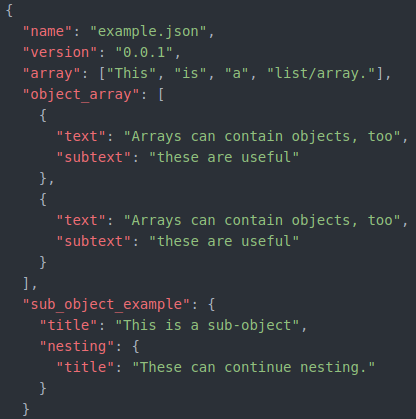
\includegraphics[width=4in]{images/Thesis_JSON.png}
    \caption{JSON excerpt from Beestream's package.json file.}
    \label{fig:json}
 \end{figure}
JSON or JavaScript Object Notation \cite{json} is a data interchange format that is heavily integrated with JavaScript.  The notation is intended to be human-readable, simple, and textual.  It is also used by JavaScript for most object representation.  It is simply constructed of objects that open with a single { (curly brace) followed by a series of comma-separated key-value pairs in the format key : value and closed by a single } (curly brace).  It can also contain lists defined by an opening [ (square bracket) followed by a list of comma separated values or objects and closed with a ] (square bracket).  Part of Beestream’s package.json can be seen in Figure \ref{fig:json} as an example of JSON. This means that JavaScript can be used for anything from data transmission or storage in a web application to human-defined configuration files for web servers and clients.  Due to its simplicity and deep integration into JavaScript, JSON is typically at the core of any JavaScript based application. \par

\subsection{Socket.io & WebSockets}
Socket.io \cite{socket} is a package distributed through NPM that utilizes the WebSocket protocol to offer bi-directional communication channels between a server and a client.  Socket.io provides valuable abstractions for the server and client to setup and communicate through WebSockets.  Socket.io is stable, performs well, and is widely used.  Beestream utilizes Socket.io for most server-client communications due to its simplicity and performance. \par

\subsection{Angular}
Angular \cite{angular} is a client-side application framework built in TypeScript.  TypeScript \cite{typescript} is a strongly typed superscript of JavaScript that compiles into plain JavaScript.  One of Angular’s primary features is its strict enforcement of the MVC architecture with modules, components, and a rendered view.  Angular seeks to provide the developer controlled access to the HTML document and a reliable and secure experience.  Because Angular controls the document, it can provide useful features such as a module-component structure, template-based rendering, and a router to render the appropriate components based on the current URL.  Angular also offers easy support for dynamic content with simple two-way data mapping from the client TypeScript to the rendered document.  Fundamentally, Angular tries to offer a reliable framework for building applications using TypeScript/JavaScript with certain stability and security guarantees.  Other frameworks, such as Vue and React, have seen wide use and can be interchanged with Angular in most applications.  Beestream uses Angular as it’s client-side framework. \par

\subsection{MongoDB}
MongoDB \cite{mongo} is a NoSQL database solution that utilizes BSON (Binary JSON) for data storage.  MongoDB provides a good read-write performance balance and allows for flexibility in the data types and formats that are stored.  Above all, MongoDB integrates well with JavaScript and returns JSON-formatted results that can be immediately accessed and used within a web server or client. \par
 \label{bkgrnd_technical}
				\section{Application Background}
				%
% bkgrnd_application.tex
%

	Our architecture was applied as part of the Beestream web application.  In order to understand the motivations for this project, the reader should have a general understanding of the Beemon project.  Beemon is a honey bee hive monitoring application that records video, audio, and temperature/humidity data at the entrance of a honeybee hive.  The recorded data is uploaded to a remote server where it can be accessed and analyzed.  As part of the Beemon project, a number of automated video and audio analytics programs were created.  These applications produce quantitative data, such as beehive arrivals and departures, from qualitative video and audio data.  When video or audio data is uploaded to the server, it is ingested into a MongoDB database and analyzed using these analytics programs.  The analysis results are included in the MongoDB database.  Beestream’s original purpose was to allow users to stream the video recorded by Beemon through a web application and comment/tag videos with interesting observations.  Given the readily available analysis, the idea was presented that Beestream could include various visualizations of the live honey bee hive data such as arrivals, departures, and temperature/humidity.  Our architecture was developed and applied to this visualization problem. \par
 \label{bkgrnd_application}

	\chapter[Objectives]{\centering Objectives} \label{objectives}
	%
% objectives.tex
%

As with most software design projects, our architecture was created to offer a reusable solution to a set of common problems.  Akin to a software design pattern or architecture, this thesis presents a general-purpose architecture to solve the common problems faced in web-based interactive data visualization applications in a general, adaptable, and reusable way.  This section will overview the common problems that inspired the creation of a common-use architecture. \par

\section{Data Scaling}
The primary limiting factor for a web-based data visualization is its platform.  Web-based data visualizations are rendered in the web browser so the scale and interactivity of a data visualization is limited by the abilities of the client’s web browser and device.  If too many data points are rendered in a single webpage or visualization, especially interactive visualizations, the experience can become laggy, unresponsive, or even cause issues with the web browser.  As a result, the application must limit the number of rendered data points within a given browser window to provide a fluid and responsive experience. This limitation creates the problem of data scaling. Data scaling refers to the process of aggregating, summarizing, or otherwise reducing the number of data points from a given input to some smaller output.  For example, if a given dataset contains five thousand unique points but the browser can only render approximately one thousand points before its performance degrades, the dataset has to be aggregated or scaled to one thousand points before visualization. \par
Ideally, the data scaling process should attempt to show as much detail in the visualization as possible, without sacrificing responsiveness and fluidity in the live visualization.  An ideal visualization application would allow the user to focus in on a subset of visualized data and view that subset in more detail.  This indicates a need for adaptable scalability.  Recall our earlier example which discussed a chart showing one thousand points aggregated from a five thousand point dataset.  Within this example, the user should be able to focus on 20\% of the dataset, equating to one thousand data points from the original dataset and two hundred data points from the aggregated set, and view all one thousand data points from the original dataset.  This illustrates adaptable data scaling, allowing the user to view a subset of the data in the greatest detail possible within the limitations of the web browser. \par
The data scaling process should also minimize impacts on the application’s loading time and performance demand on the client’s device.  If the data scaling process improves the fluidity of the data visualization but causes the application to take an additional ten seconds to load a dataset, other visualization or scaling means should be considered.  Alternative scaling methods should usually be considered if they affect the loading time such that additional latency accommodations should be made.  Specifically, if the addition of a certain data scaling method causes the system to take more than 10 seconds, either a progress bar must be added or data scaling must be optimized \cite{doet, aboutface}.  Another concern arises if the data scaling process is executed on the client’s web browser where the speed of the scaling process will depend on the capabilities of the client’s device.  In this case the scaling process will could potentially affect the client’s device performance and, in the worst case, cause the web browser to become unresponsive. In the end, the primary goal of data scaling is to improve the responsiveness of an in-browser data visualization without greatly compromising detail and to do so with minimal effect on the performance of the rest of the application. \par

\section{Data Sources}
Data sources are a common avenue for change in highly data-dependent web applications. An application may be paired with one or more database solution for local data storage and might even acquire data from remote sources through external web APIs.  As such, any architecture that seeks to generally accommodate data visualization must remain decoupled from data sources. An architecture shouldn’t be coupled to one database solution or remote API interface.  For example, a web application to provide weather data could either use a local MongoDB database for all of its data needs or it could use an SQL-based database to provide weather forecasts and acquire real-time temperature and wind data from a remote web API.  In this case, the architecture should allow the software developer to define these modes of data acquisition generically.  It is also ideal to encapsulate these data source and data interactions as they are likely to change later.  Given that web API’s tend to change format or location, data sources should have a clear location for change which is isolated from the rest of the application. The architecture can also use this abstraction to enforce solutions to other common problems such as data scaling and transmission. \par

\section{Data Transmission}
Server to client data transmission is a core function of any web-based data visualization application.  Any web application that wishes to visualize data on a web client must first transmit that visualizable data from a web server to the client. Different modes for data communication exist and must be accomodated.  The two primary modes for communication over the web are through HTTP requests and WebSockets.  Both of these methods have seen widespread use and thus both must be accommodated and leveraged by any general-purpose architecture.  The issue of data transmission is an issue of encapsulation.  The mode of data transmission should be encapsulated to ensure that the architecture is flexible to the needs of a developer.   In some extreme cases, an application may pivot from a HTTP request based data transmission system to a WebSocket-based transmission system or vice versa.  These changes should be modular and isolated from the remainder of the application.  An architecture should encapsulate data transmission methods into one location and make an effort to decouple data transmission from any control logic for data acquisition. \par
Server to client data transmission is important, but if the data received by the client isn’t in a format comprehensible by the client, the data is useless.  The server and the client should both obey some standard format for data communications such that a change on one end of the data transmission should not break functionality on the other end.  For example, if the name of a data field changes and the client is tightly coupled to the naming scheme of transmitted data fields, the client will break.  This can also lead to errors that are hard to debug, where data is received by the client but not interpreted properly.  As such, any architecture should include a means of predictable data formatting such that the server can rely on a certain request format from the client and the client can rely on a certain response format from the server.  That being said, the server and client should adapt to new datasets with minimal changes. Data transmission formatting is a difficult problem, but the creation of a standard can aid in writing adaptable code. \par
Beyond data transmission formatting, the server must also optimize its responses for size efficiency and quick transmission.  This problem is twofold, responses should be as small as possible and renderable data should be sent to the client as quickly as possible.  The response size will be somewhat minimized by scaling data on the server-side as described in section 4.1.  By sending only the points that will be rendered by the client, the server can avoid transmitting unnecessary data.  As for renderable data, an architecture should have a means of prioritizing the fastest renderable response.  Data transmission not only relies on format, but also on speed and size. \par

\section{Dataset Filtering and Security}
Data security is an important issue for any web application, specifically for applications focused entirely around the transmission and visualization of data from a centralized provider. Any architecture can make simple architectural decisions to prevent common mistakes relating to data security.  One of the primary problems facing web servers is unsanitized user input.  In the case of any data visualization application, the client will issue a request to the server for data.  An architecture should enforce a standard method for request validation and ensure that the client doesn’t request or receive sensitive datasets. \par

\section{Charting Package Agnosticism}
The field of web development is filled with varying solutions for interactive and non-interactive chart creation, rendering, population, and management \cite{d3homepage, chartjs, highcharts, c3js, bokehjs}.  These libraries often focus on either specific differentiating features \cite{chartjs, highcharts}, simplicity \cite{chartjs, highcharts}, backend optimizations or accomodations \cite{bokehjs}, special dynamicity, or adaptability and flexibility \cite{d3homepage, c3js}. Charting libraries also appear, change, and disappear frequently as the area of web-based data visualization continues to grow and evolve.  As a result, an architecture for generalized web-based data visualization should be charting package/platform agnostic.  Specifically, charts should encapsulated.  As such, charts should be entirely separate from data acquisition and control logic for the data visualization page.  Charts still need to be able to dynamically request data for visualization and must also be updated when new data is available.  Finally, charts must be able to exist independently of one another, but must also have a means of interaction if the developer desires.  In essence, charts need to be individually encapsulated and defined in order to be charting platform agnostic, but there must exist a standardized “gatekeeper” or “driver” that interacts with the server and updates the charts.  The developer should be able to choose any charting package(s) of their choice and implement them freely while still obeying the architecture.  Ideally, charting package(s) and charts themselves should be easily interchangeable.  \par

\section{Dataset Loading and Processing}
A chart should only be rendered by the client if the server has provided all the necessary datasets.  It would seem logically obvious that a chart without data should not be show, but this adds certain requirements to chart encapsulation.  Given that a page may contain multiple charts, each chart must have a means of broadcasting the datasets it needs in order to be rendered.  It should be hidden until those datasets are provided.  As such, driver application code must include logic to check dataset availability, request only the necessary datasets, process the response, and only render charts which have all dataset requirements met. \par
 \label{objectives}

	\chapter[Methodology]{\centering Methodology} \label{methods}
	%
% methods_intro.tex
%

Methodology \label{methods_intro}
		\section{Server Side Architecture}
		%
% methods_server_side.tex
%

The server-side architecture relies on one primary abstraction for datapaths, a standardized format for different data “channels,” and a configuration file.  These abstractions are utilized by a single server-side driver layer to handle client data requests.  The driver will use these abstractions to solve the issues of data scaling, data sources, and dataset filtering and security.  Specifically, the driver should capture client requests and use a configuration file parameter to validate the request.  If a client requests a dataset that isn’t available or the client isn’t permitted to access, the configuration file validation should filter out that dataset from the request. Next, the driver should use datapaths to acquire data across various data channels and form a response to the client.  This data acquisition process is visualized in Figure \ref{fig:server-side-request} with a concrete examle of a request's processing flow.  To equate this system to an MVC (Model-View-Controller) architecture: the driver is the server’s controller, the datapaths are the controller’s interface to the model, the models are represented by data channels, and the client is the view.  Data channels are a construct available within data paths to represent different models or data sources that are accessed simultaneously and transparently to the driver.  Finally, the configuration file(s) allow the developer freedom to govern dataset availability. \par
  \begin{figure}
    \centering
    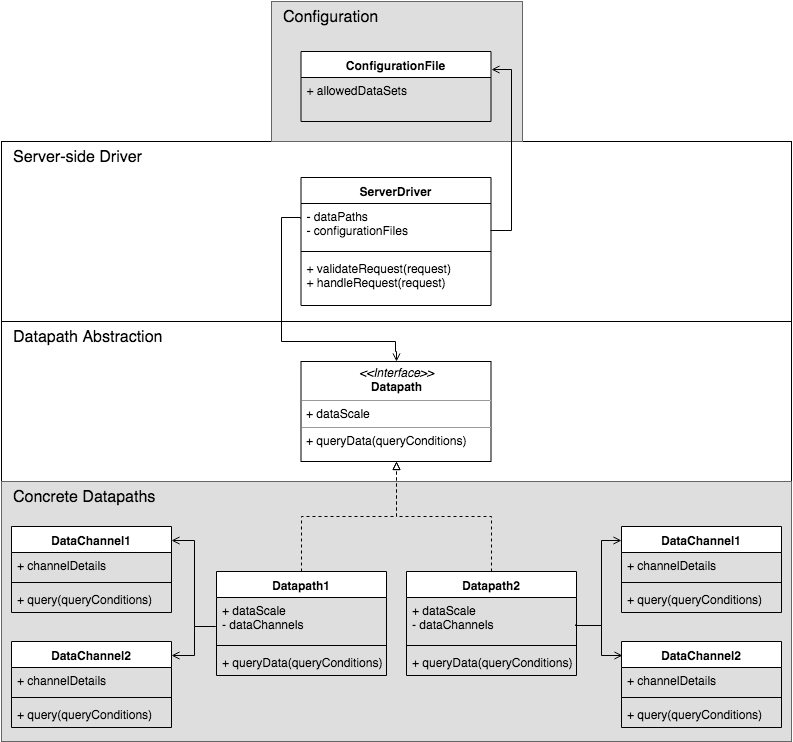
\includegraphics[width=6in]{images/ServerSideClassDiagram.png}
    \caption{Server-Side Class Diagram}
    \label{fig:server-side-class}
 \end{figure}
 \begin{figure}
   \centering
   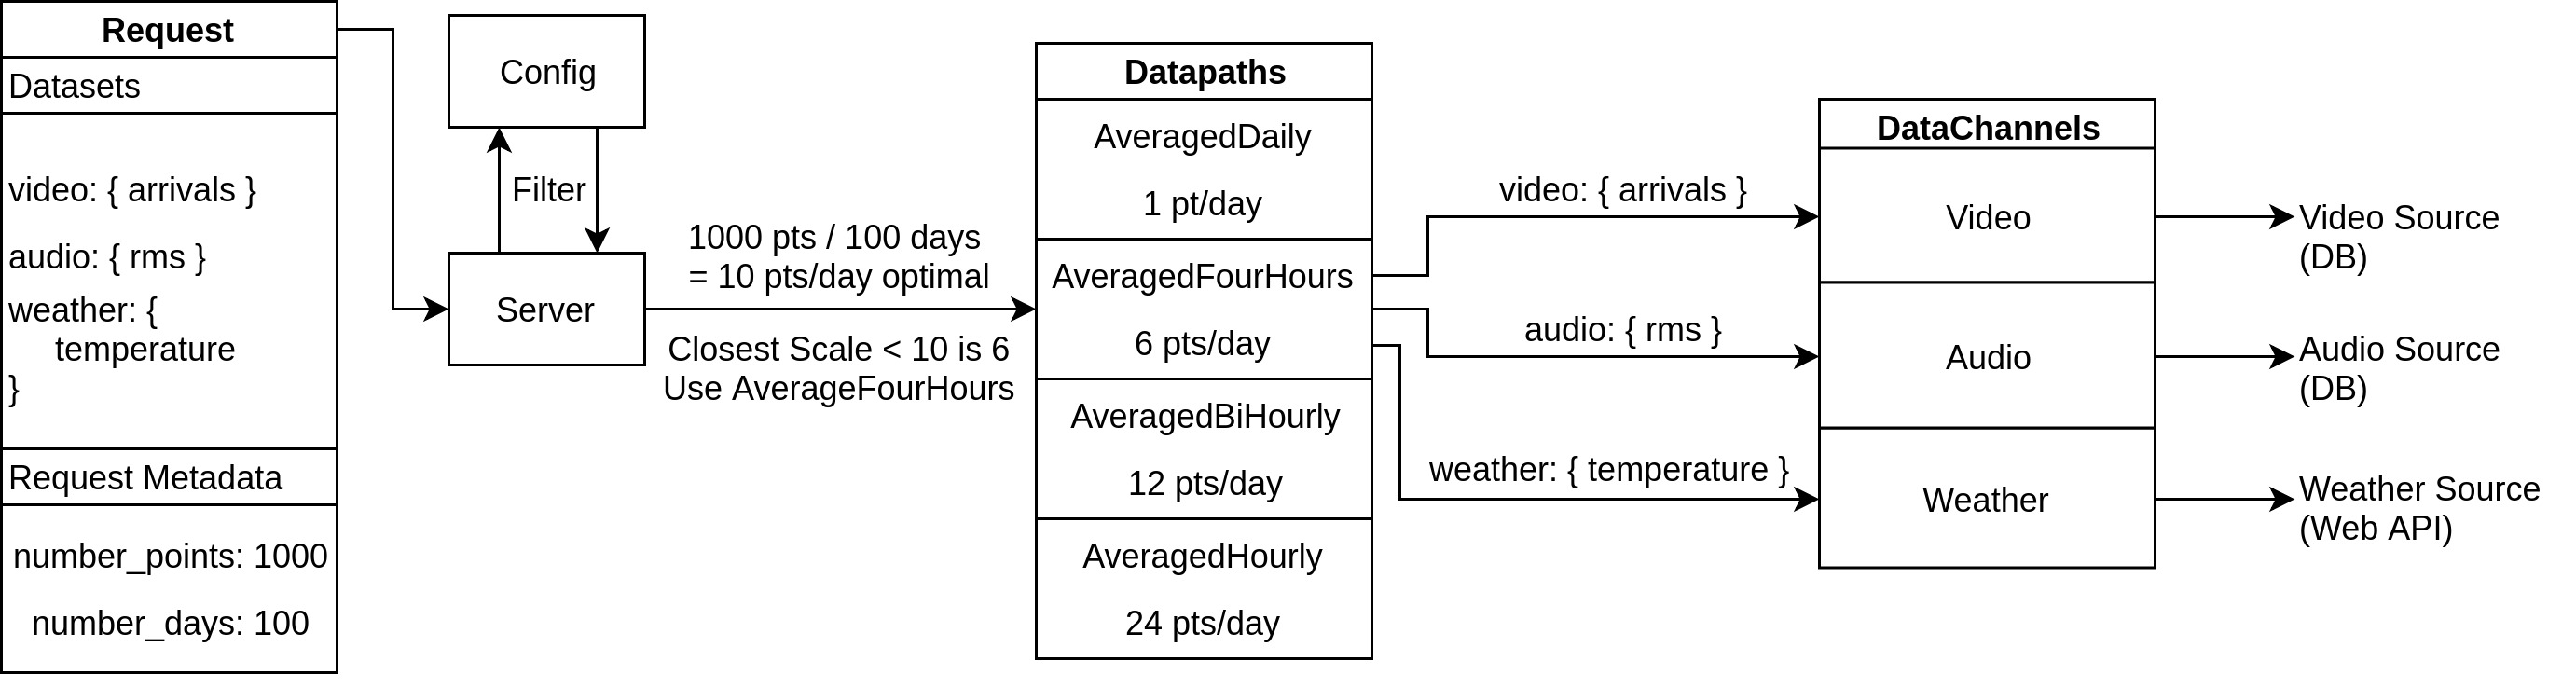
\includegraphics[width=6in]{images/DatapathDataChannelExample.jpg}
   \caption{Request Process Flow}
   \centering{The server receives a request for 1000 data points across 100 days.  It filters this request through the configuration file, selects the optimal datapath by data scale, and queries from that datapath.  The datapath splits the request by channel and queries the data channels, for example \textit{video: \{ arrivals \}} indicates the arrivals dataset should be quired from the video data channel.}
   \label{fig:server-side-request}
 \end{figure}
The server-side implementation is separated into two key segments: driver code and modular code.  This division can be seen in Figure \ref{fig:server-side-class}.  In the figure, all driver code is found within white blocks and all modular code can be found within grey blocks.  The goal of modular segments is to encapsulate the primary modes of change for the server-side.  This means that the developer only needs to define driver code once, but may revise, add, or remove modular elements as required. The driver is responsible for processing client requests, filtering them using configuration files, and responding to requests using data from datapaths.  Within this system, data scaling and data sources are encapsulated within datapaths and dataset filters are encapsulated within the configuration file layer. \par

\subsection{Datapaths}
Datapaths are the primary server-side abstraction built specifically to solve the issues of data scaling and data sources.  The goal of a given datapath is to encapsulate data accesses and scaling within a common interface such that the driver can dynamically interact with different datapaths.  The developer can define multiple datapaths by extending the datapath interface.  The datapath interface requires the developer to define a field which informs the driver of the datapath’s data scale and a function to query data given query conditions as input.  The query function should handle all data acquisition from one or more data channels and any data aggregation.  The dataScale field should export some common metric to measure scale such as items returned per unit, for example the number of data points returned per day.  The driver will import multiple datapaths and use their dataScales to determine which to use when handling a request. \par
When the developer implements a concrete datapath, they can handle data scaling as desired.  For example, a certain dataset may contain one thousand points and include a datapath to scale this data to only one hundred points.  This datapath could aggregate the data in groups of ten by taking the minimum, maximum, average, median, etc.  The proper aggregation method will be depend on the data and the desired result.  This is the reason behind the datapath system, the developer is free to aggregate data sets to different scales, and using different methods of aggregation. \par
Concerning concrete implementation of this architectural element, Beestream implements datapaths by making use of JavaScript’s module system.  Each datapath is defined as a module that exports a query function and a dataScale value.  All datapaths are placed in a single folder within the server-side project code.  The server’s driver code dynamically imports all files within the datapaths folder and will save any file that matches the datapath interface to a list.  The driver will validate that each imported file exports a query function and a dataScale value before saving it to a list of usable datapaths.  This system behaves almost identically to an object-oriented interface and concrete class system, only the driver must enforce the interface explicitly.  Whenever the server receives a request, it will find the dataScale that will provide a number of points closest to the desired number of points.  It will call this datapath’s query function to access data to be delivered to the client.  Beestream’s datapaths provide different data scaling levels using multiple MongoDB aggregate views.  Different views aggregate time-series data hourly, bi-hourly, and daily.  These MongoDB views perform better than querying the full dataset and aggregating in JavaScript within the datapath. \par

\subsection{Data Channels}
Datapaths offer the driver a common interface to access different data sources.  Each datapath can draw data from numerous different data channels.  A data channel represents a single data source.  Much like a television or radio channel allows an individual to access different data through the same medium, the datapath can query from multiple channels to get different data from different datasets through the same interface.  The primary goal of data channels is to separate the driver from various data sources.  This is accomplished by allowing the driver to ask for datasets from a channel by nesting the dataset within a JSON object for that chanel.  For example, when the driver is asked for a temperature value which exists on the weather data source, it will request “weather: {temperature}”.  The datapath will interpret this as a request to query for the temperature dataset from the weather channel as visualized in Figure Figure \ref{fig:server-side-request}.  When the driver receives a result from the dataset, it will receive “temperature” as desired without the knowledge that the dataset had to be queried from a different data source. \par
Data channels reside within modular code, so they are not strictly enforced in the architecture.  The primary goal of data channels is to suggest that different data sources be encapsulated for reuse and feature a common interface.  Datapaths are a suggested feature, but ultimately the developer who defines various datapaths should identify their different data sources and encapsulate them as is appropriate.  If the same data sources are used in multiple places, then they should likely be encapsulated and reused.  If a data source is only used once, then it likely doesn’t need encapsulation.  Data sources’ interfaces can also vary greatly, encompassing various database solutions and web APIs.  As a result, it would be difficult to architecturally require a single interface for data sources, so this choice is left up to the developer writing the datapaths.  Code reuse and modularity is still encouraged. \par
In Beestream’s concrete implementation of data channels, data channels are not expressly abstracted.  Beestream only uses three MongoDB collections as data sources, so they are directly queried using the same interfacing package, called Mongoose.  All queries are executed in parallel using the Async package.  If the project wanted to include data from a web API, that would likely be added through an abstraction to create the same interface as a Mongoose collection following the suggestion that data channels should share an interface if possible. \par

\subsection{Configuration Files}
Our architecture includes configuration files specifically for the purpose of dataset filtering and data security.  Configuration files should be used to define a list of allowed datasets.  The server driver should check all client requests against the allowed datasets list and only permit the client to access datasets present on that list and in the data source.  In essence, the driver should filter all requests using the allowed datasets list before completing a query.  Any datasets that are not “allowed” should be filtered out of the request before a query is made.  Using this method, we ensure that the client is only able to access datasets that the developer expressly allows. \par
Beestream’s concrete configuration file implementation involves named configuration files containing a JSON configuration object.  This JSON entry contains an object that lists the various datasets available for access across multiple data channels.  The server will check the NODE\_ENV system environment variable and will import either a “development” configuration file or a “production” configuration file, permitting the use of two different allowed datasets lists for development or production environments.  Once the correct file is included, the server driver can filter out disallowed request fields as needed. \par
 \label{methods_server_side}
		\section{Data Transmission}
		%
% methods_data_transmission.tex
%

\subsection{Server-Client Handshake}
Any web-based data visualization involves some communication between the server and the client in the form of requests for data and responses including transmitted data.  In order to effectively communicate and exchange visualizable data, the server and the client must “speak a common language” by offering requests and responses in a predictable format.  Our architecture allows the client and the server to accommodate changes to the available dataset list while still maintaining a standard communication format.  This is accomplished using a simple server-client handshake as is visualized in Figure \ref{fig:server-client-handshake}.  The handshake opens with the client page loading and emitting a connection event.  The server catches this event and generates a list of available datasets typically populated using a configuration file and/or database query.  This list is then transmitted back to the client.  The client receives the list and since it knows what datasets are available for querying, it will form a response.  The server filters this request using it’s configuration data to prevent unpermitted data accesses.  The server will then query using the filtered dataset list and form a response to the client.  The response will be formatted such that each requested dataset is a JSON object key used to access a list of data items for that data set.  Finally, the client receives the data and can dynamically interpret it using the dataset list that it has received at the beginning of the handshake. This simple handshake system allows the client and server to dynamically include new datasets or remove old datasets without codebase changes. \par
\begin{figure}
    \centering
    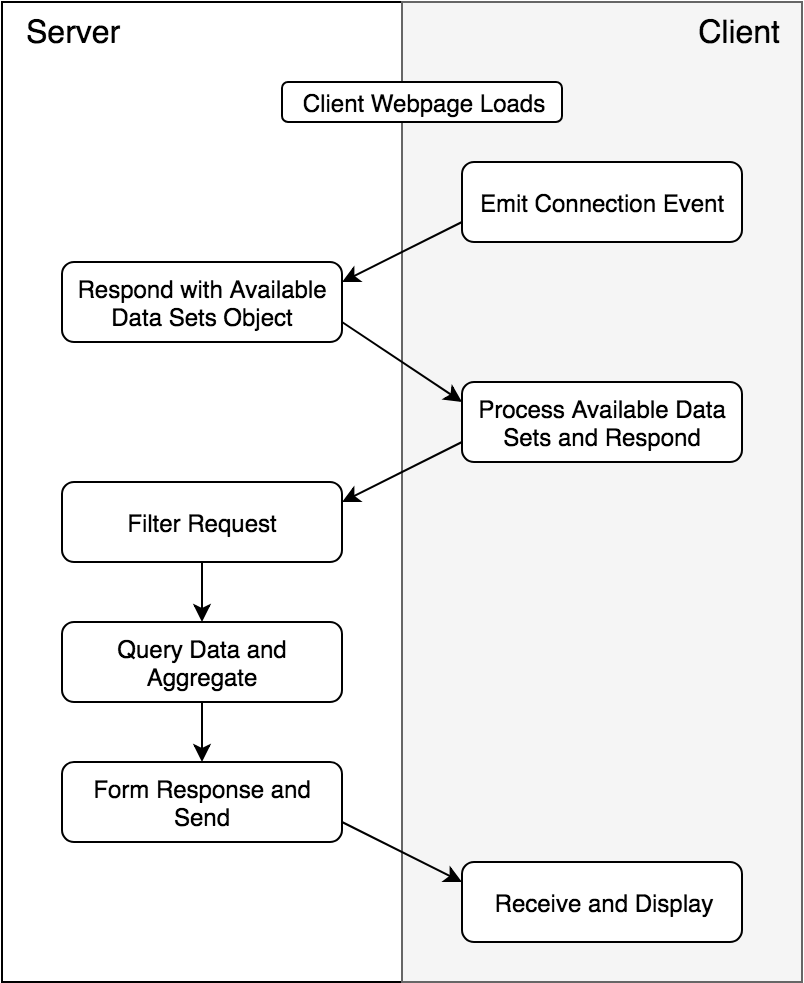
\includegraphics[width=4in]{images/ServerClientHandshake.png}
    \caption{Server-Client Handshake}
    \label{fig:server-client-handshake}
 \end{figure}
Beestream includes a concrete implementation of this data transmission system.  The implementation utilizes Socket.io to handle bidirectional communications.  All data is transmitted in JSON format.  The implementation follows the architecture almost directly, differing only in the original dataset list handshake step.  During this step, the server not only responds with a list of available data sets, but also a list of available datetimes and other fields necessary to populate a data selection widget.  The client will then transmit a set of selected datasets as well as a range of data points to the client in the next response.  The format for this communication is standardized throughout the application.  Using this method, we can allow the user to filter the dataset and form their data request. \par
 \label{methods_data_transmission}
		\section{Client Side Architecture}
		%
% methods_data_transmission.tex
%

Our client-side architecture consists of one primary abstraction for chart components.  By abstracting chart components behind a common interface, we can accomplish charting platform agnosticism and create a predictable life cycle governing the loading of datasets and rendering of charts.  Our client, much like the server, has a “driver” component.  The driver component should be static as the architecture seeks to encapsulate all common avenues of change within the chart components.  The driver’s goal is to handle server-client communications and enable the user to query data as the developer sees appropriate.  The driver can simply load a default query from the server or include a query builder for the client’s use.  The developer can choose which functionality best suits their needs, but the application should utilize the common chart component interface to interact with charts. \par
The client-side design and implementation are quite simple. The following sections will overview each feature, discuss the architectural decisions, and present our implementation.  The client-side architecture draws more direct inspiration from Angular’s component system, however it is easily implementable across different client-side frameworks or even in framework-less client-side code. \par

\subsection{Chart Components}
Our primary client-side abstraction defines a common interface for charts.  Each chart component should define a single renderable chart, although the developer can freely define multiple charts, widgets, or other data visualization features within a single component.  A“single component - single chart” policy is recommended to improve modularity but it is not strictly enforced.  Each charting component must implement a common interface, visualized in Figure 5.4.1 as the \textit{ChartComponent} interface. This interface requires the charting component to have a list of required datasets, a function to access that list, and a function to update the chart’s data.  This interface allows the charting components to be loosely coupled with the driver.  Once the driver has received data, it obtains a list of a chart component’s required datasets, validates that it can provide all the required datasets, and calls that components lifecycle hook to update it (\textit{updateChart} in \ref{fig:client-side-class}). \par
By interacting with charting components only through a common interface, we eliminate any coupling between data acquisition control logic and chart rendering.  Our architecture is reminiscent of an observer pattern.  The client driver will serve only one primary purpose: to query data from the server and ingest that data.  Once it has obtained that data, it “notifies” the chart components of updated data using their \textit{updateChart} lifecycle hook.  The chart components, in this instance, are our observers, waiting for changes from the driver.  This system allows the developer to define data acquisition code in the driver once, and modularly add charting components.  This also introduces the possibility of dynamic chart components that allow the user to select what data is shown/compared within the chart component. \par
Chart components also allow the data acquisition “business logic” to be entirely independent and unaware of the charting libraries in use.  This allows our architecture to provide complete charting platform agnosticism.  The developer can change charting libraries by simply writing new charting components that utilize a new library.  A single client page can even include multiple charts from multiple charting libraries, all encapsulated within their own chart components.  All of this can be achieved with no change to the data acquisition/business logic in the driver. \par
Beestream’s client is implemented using Angular as a client-side framework.  Angular’s framework includes constructs for modules and components to define functionality and pages. Angular also utilizes Typescript which provides class and inheritance constructs.  This allows us to implement the client-side architecture shown in Figure \ref{fig:client-side-class} almost directly.  The implementation includes a single module for the charting page, which declares a single driver component and all registered chart components.  The driver has knowledge of all chart components as part of its renderable template.  The driver holds all server-client interaction logic and includes a small widget to allow the user to build simple queries.  Angular renders pages by calling a series of lifecycle hooks.  These lifecycle hooks are also intercepted by the driver.  Once the page is initialized, as is signaled by the \textit{afterViewInit} lifecycle hook, chart components are rendered.  These charting components can determine their own behavior after initial rendering, although in our case they simple render as hidden.  Each chart component is implemented as a separate Angular component that implements a ChartComponent interface.  As such, the driver is guaranteed to have access to a method to update the chart and a method to list required datasets.  Overall, our implementation maps almost directly to the defined architecture. \par

\begin{figure}
  \centering
  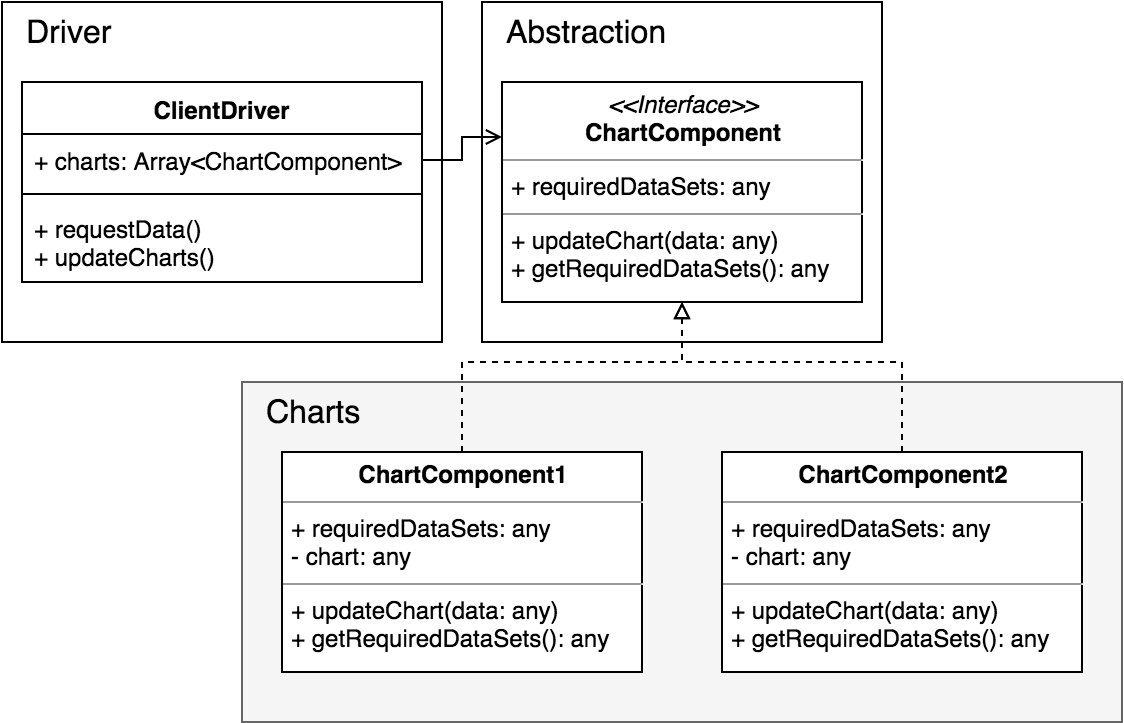
\includegraphics[width=6in]{images/ClientSide.png}
  \caption{Client Side Class Diagram}
  \label{fig:client-side-class}
\end{figure}

\subsection{Dataset Request Flow}

Our architecture presents a simple dataset request flow which allows each charting component to request datasets.  Each chart will only be updated and rendered if the required datasets are available.  This offers the guarantee that empty charts will not be rendered if data is missing, avoiding any errors associated with rendering an empty chart.  This behavior is enforced by using the simple handshake shown in Figure \ref{fig:client-dataset-request} before any data request is made and the handshake shown in Figure \ref{fig:client-update-flow} after data is received.  These handshakes must be enforced by the developer-defined client driver.  Using these handshakes, the driver can ensure that it queires only the necessary datasets from the server to reduce data transmission size and render only those charts whose data is available. \par
\begin{figure}
  \centering
  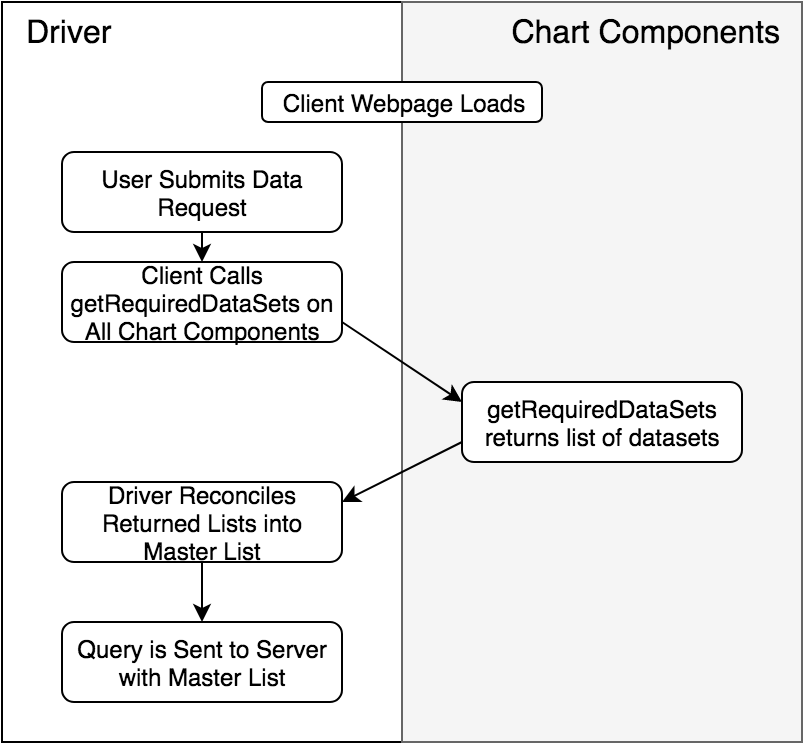
\includegraphics[width=4in]{images/ClientDatasetRequestFlow.png}
  \caption{Client Dataset Request Flowchart}
  \label{fig:client-dataset-request}
\end{figure}

\begin{figure}
   \centering
   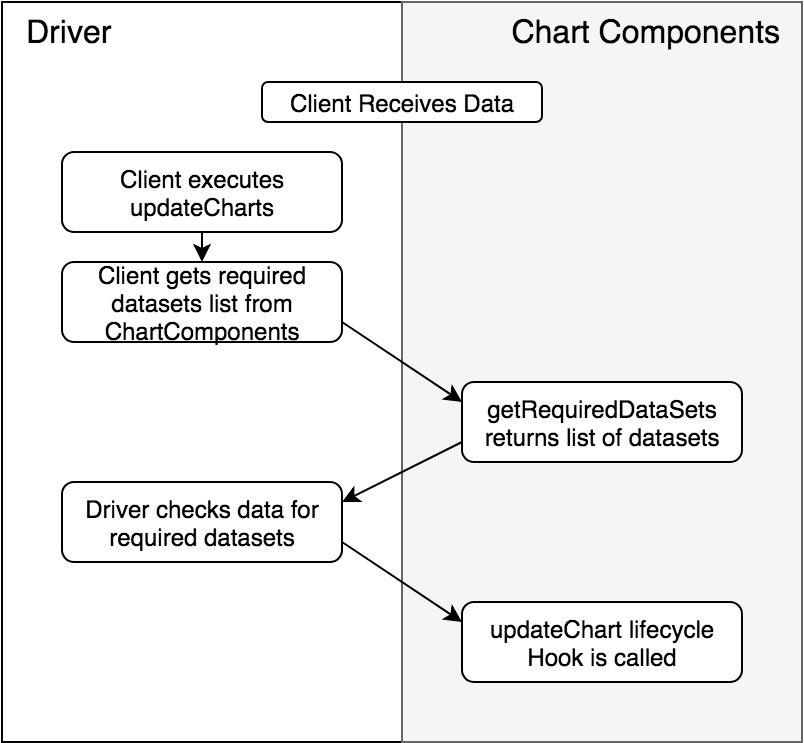
\includegraphics[width=4in]{images/ClientChartUpdateFlow.png}
   \caption{Client Chart Update Flowchart}
   \label{fig:client-update-flow}
\end{figure}

The first handshake occurs after rendering the page, rendering chart components, and only after the driver has received the initial list of available datasets from the server.  Before the client driver sends a data request to the server, it will poll every chart component for its required datasets.  Using this information, the client driver will populate a list of all unique required datasets.  This list should be cross-checked with the list of available datasets sent from the server.  After any unavailable datasets are removed from the list, it will be used as a parameter in the data request.  This step ensures that the client requests only the data it needs to render charts, avoiding unnecessary data transmission. \par
The second handshake occurs when the client driver receives data back from the client after issuing a data request.  In this handshake, the driver will iterate through all chart components.  The driver will check each chart component’s required datasets list and, if all dataset needs are met, it will call that component’s update lifecycle hook and pass it the relevant updated data.  If all required datasets are not available, the update hook will not be called.  If the developer desires, they can add a “missing data” lifecycle hook to the chart component interface and call this hook if required datasets are not present.  This handshake ensures that charts are only rendered if all required data is present. \par

\subsection{Lifecycle Control}

In sections 5.4.1 and 5.4.2, we’ve frequently referenced a chart “lifecycle.”  Our architecture defines a certain lifecycle for rendered chart components through both implicit driver logic and the chart component interface.  The client driver ultimately controls when and how charts are rendered and delivered data.  As such, the driver controls the lifecycle of the chart components.  As discussed in section 5.4.2, each chart is only rendered and updated with data if the required data is available.  These extra steps can be seen in figure \ref{fig:client-lifecycle-flow}.  The handshakes discussed in 5.4.2 define a simple lifecycle for a chart, however our driver can more strictly enforce a lifecycle through the use of Angular’s lifecycle hooks. \par
\begin{figure}
    \centering
    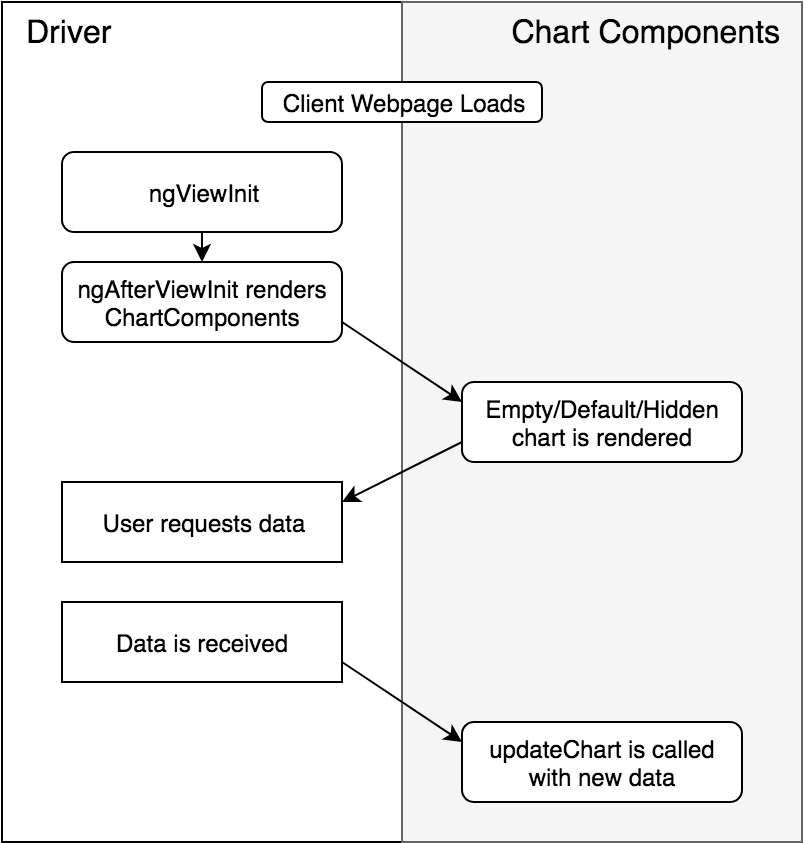
\includegraphics[width=4in]{images/ClientLifecycle.png}
    \caption{Client Chart Lifecycle Flowchart}
    \label{fig:client-lifecycle-flow}
\end{figure}
Depending on the charting library, charts can be dynamically generated, populated, updated, and destroyed.  In Beestream’s implementation, C3.js charts are utilized.  In this library, charts are bound to a single HTML element after the page is fully rendered.  As such, each chart component shouldn’t be rendered until after the webpage is rendered.  This is enforced by having each chart component using C3.js implement the \textit{ngAfterViewInit} lifecycle hook.  The chart can render at this time, but it doesn’t need to be shown yet because it hasn’t been given data.  The client driver is responsible for handling this part of the lifecycle.  As a result, Beestream’s chart components must respect Angular’s lifecycle for chart rendering and the client driver’s lifecycle for chart display and population.  The chart is “rendered” but hidden until the client driver allows it to populate. \par
 \label{methods_client_side}

	\chapter[Results]{\centering Results} \label{results}
	%
% results_intro.tex
%

Our architecture sought to provide a generalized, adaptable, and extensible solution to the problem of web-based data visualization.  In order to demonstrate the practicality effectiveness of our architecture, we’ll overview the procedure to extend the Beestream web application.  The following sections will cover different common avenues of change for web-based data visualization applications and how our architecture accommodates these changes.  In most cases, the Beestream application will be discussed as an example. \par
 \label{results_intro}
		\section{BeeStream Application}
		%
% results_application.tex
%
One of the primary results of our architectural design is the BeeStream web application.  BeeStream was built using our architecture with the purpose of visualizing automated honeybee hive analytics data.  Figure \ref{fig:beestream-screenshot} shows Beestream's interface with data loaded.  We've made use of the architecture's modularity for data sources/channels, datapaths for data scaling, data filtering, data transmission protocols, charting component encapsulation, and dataset loading/missing data prevention.  BeeStream was built using the MEAN (MongoDB, Express, Angular, Node.js) web stack and illustrates how the architecture can leverage modern fullstack JavaScript's capabilities.  \par
\begin{figure}
  \centering
  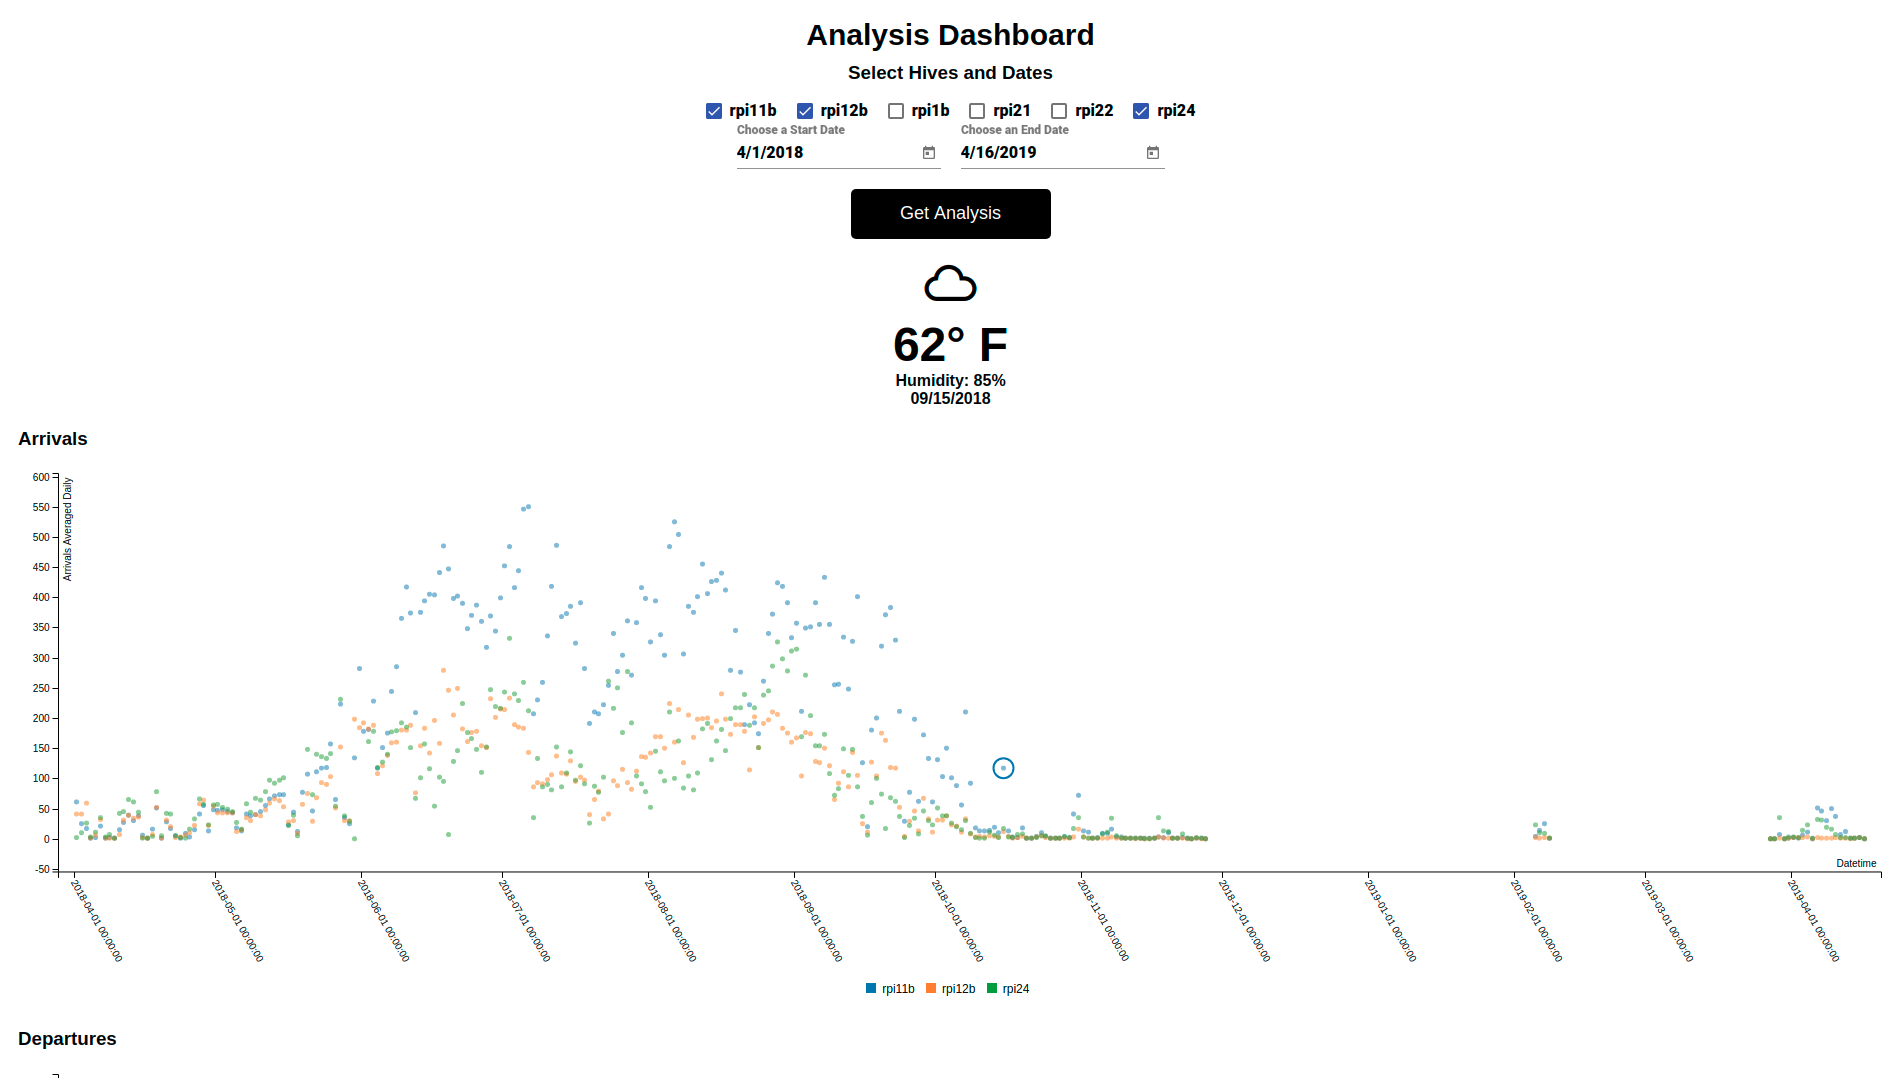
\includegraphics[width=6in]{images/beestream_screenshot.png}
  \caption{Beestream Screenshot}
  \label{fig:beestream-screenshot}
\end{figure}
Our archtectural implementation is also evident in the rendered web client.  The webpage is divided into a client driver and a series of rendered chart components as can be seen in Figure \ref{fig:beestream-screenshot-annotated}.  The client driver handles server-client communications, data filtering and requests, and the chart components' lifecycles as defined in our architecture.  Each of the chart components is dynamically rendered and populated only when data is present.  In our implementation, we chose to use C3.js \cite{c3js}, a package built on top of D3.js \cite{d3homepage} for our charting library.  As you can see in Figure \ref{fig:beestream-screenshot-annotated}, BeeStream includes a number of charts as well as a non-chart component, although the non-chart component is built to extent \textit{ChartComponent} so the driver doesn't know that this \textit{ChartComponent} doesn't define a chart.  This non-chart component is a weather widget shows the weather conditions for the point selected on the charts.  All charts use the driver to synchronize their currently selected point by having notifying the driver of a new selected point.  The driver distributes this notification to all \textit{ChartComponents}.
\begin{figure}
  \centering
  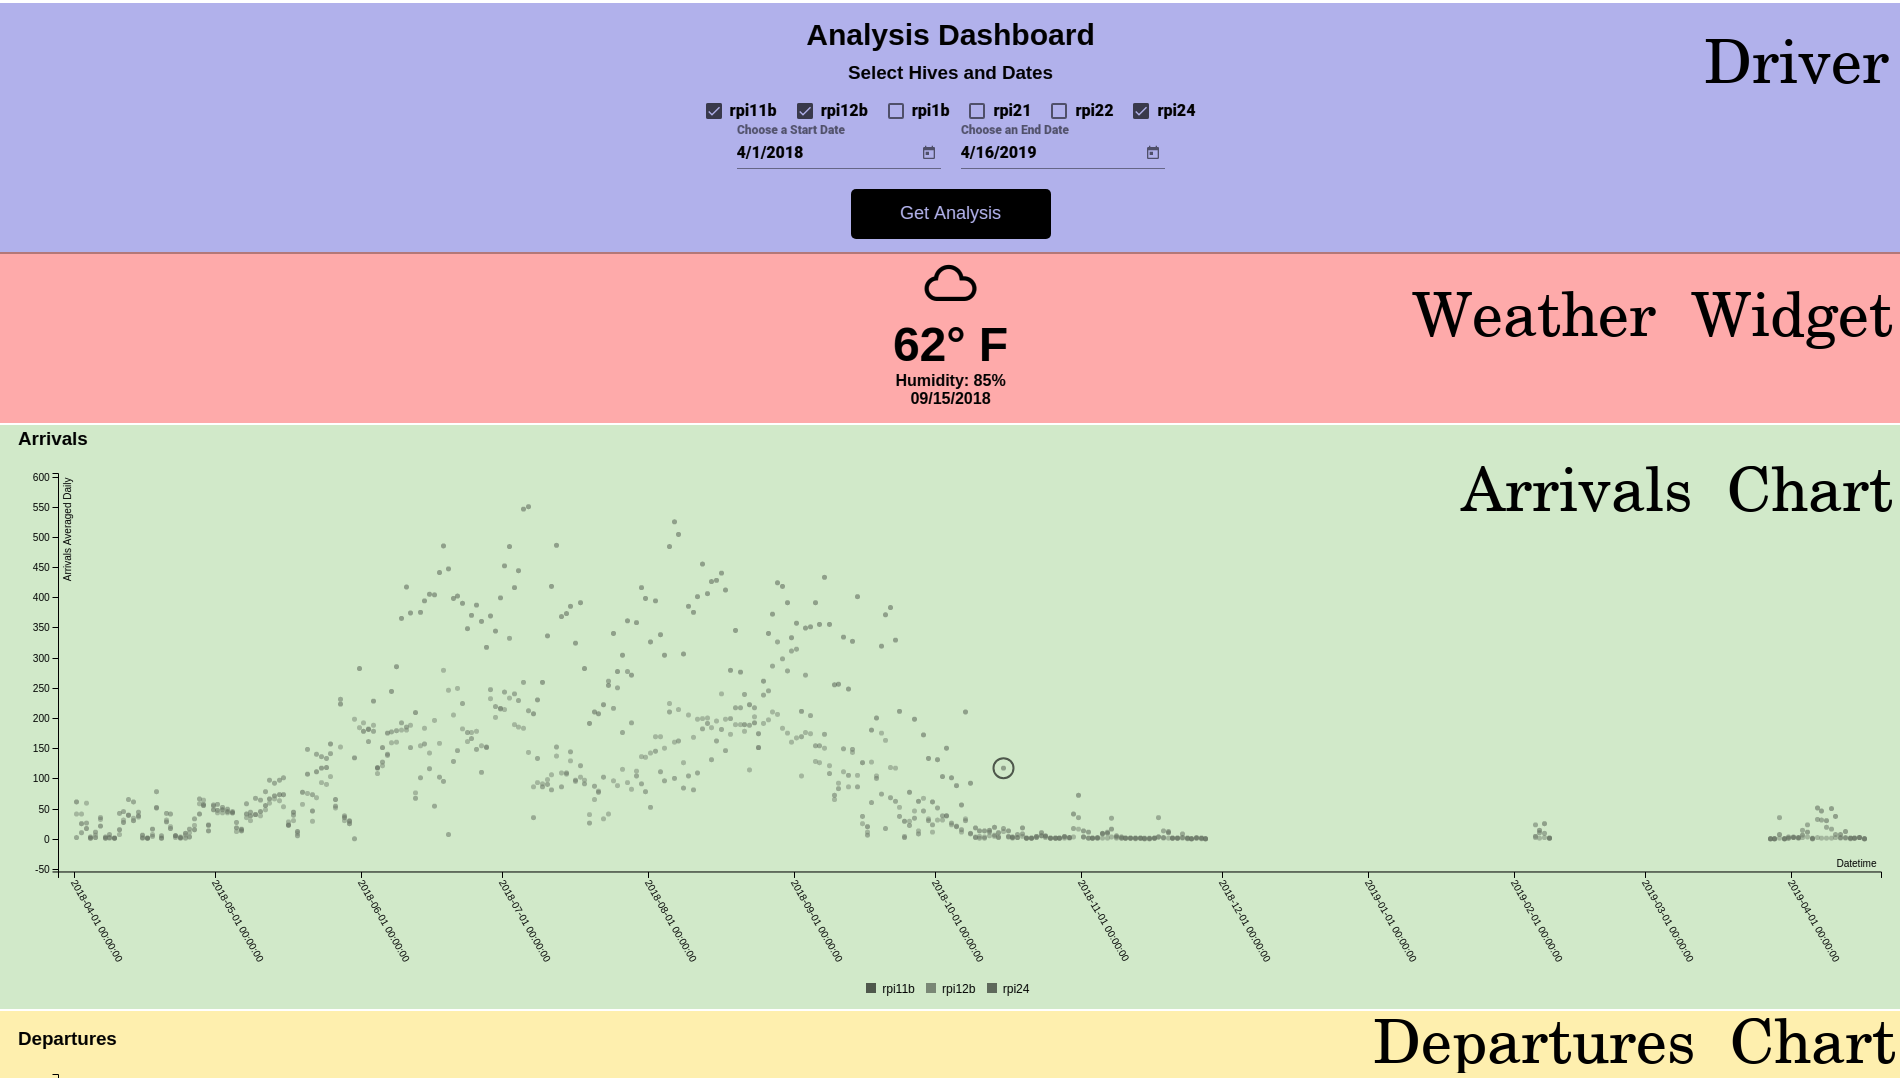
\includegraphics[width=6in]{images/beestream_screenshot_annotated.png}
  \caption{Beestream Screenshot with Annotations}
  \label{fig:beestream-screenshot-annotated}
\end{figure}
 \label{results_application}
		\section{Server Side Extension}
		%
% results_server.tex
%

\subsection{Adding a Dataset}

One of the most common avenues for change in any data visualization application is the data in use.  In our architecture, datasets are acquired from different data sources/paths through datapaths.  In order to provide a new dataset, the developer should verify that their datapaths have access to this dataset.  If all datapaths simply query dynamically from a database based on request parameters and that database contains the new dataset, the datapaths should have access to the new dataset.  If queries are not dynamically built, then the developer will have to add the new dataset to all datapaths that don’t include it.  By writing dynamic datapaths, some work can be avoided when adding new datasets.  Once all datapaths have access to the new dataset, the developer has to add that dataset to the allowed datasets list in their configuration file.  As a general security measure, datasets have to be whitelisted in order to be included in visualizations, which is addressed in this final step.  After this step, the new dataset should be available to the client and can be requested by a chart.  So, in conclusion, in order to add a new dataset, the developer needs to validate that the dataset is available to all datapaths and that it is present in the allowed datasets list. \par

\subsection{Adding a Datapath}
Another common avenue of change lies in the datapaths themselves.  Each datapath defines a data scale and data aggregation method through which the available datasets can be viewed.  A common reason to add a datapath would be to accommodate different data focus levels.  For example, if data is scaled by time, an application may include a data scale of 1 point per day and 1 point per hour.  If the developer finds that users often query a datetime range such that aggregating the points bi-hourly would be more appropriate, they can add a datapath for that data scale. In this case, the developer need only define a new datapath that queries and aggregates data at a new scale and place it in the datapaths folder.  When the server is restarted, the new datapath will be dynamically loaded and utilized when appropriate. \par

\subsection{New Data Channels/Sources}
In our architecture, different data sources are loosely encapsulated within data channels.  These data channels, as discussed in section 5.2.2, represent a single source of data that could be a database collection/table, a web API hook, or any real source of data.  Data channels should provide some unified interface.  It is highly likely that during the lifetime of a data visualization web application, the developer may want to add a new table/collection, change database solutions, or have to adapt to a change in a web API.  As such, data channels are encapsulated within their respective datapaths and can be easily added or updated.  In order to add a new data channel, the developer must first revise datapaths.  Each datapath that needs to have access to the new data channel should be revised to include code to query the new data channel.  Keep in mind that the data channel accessing code can be defined once and reused by all data paths as desired.  Once complete, they must add the new data channel’s available data sets to the allowed datasets list in their configuration file.  Once the server is restarted, the new data channel and all contained datasets will be available to the client. \par
 \label{results_server}
		\section{Client Side Extension}
		%
% results_client.tex
%

\subsection{Adding a Chart}

The most common avenue of change on the client is charts.  It is very likely that, during the lifetime of a data visualization web application, the developer will want to add, remove, or modify different charts and visualizations.  Our architecture encapsulates this common mode of change using the chart component interface.  If the developer wishes to add or remove a chart, they need only define a new chart component which requests the necessary datasets and draws the desired visualization.  In Beestream and other Angular-based applications, it is also necessary to add this component to the client module and the client driver’s list of imported chart components and template.  Once complete, the new visualization(s) will be drawn whenever the required datasets are available.  Chart can also be modified easily as they are encapsulated within modular components.  This component system also permits some dynamic behavior, allowing the driver to dynamically show/hide different charts while the webpage is loaded.  By encapsulating charts, they can be added, removed, updated, and dynamically shown/hidden. \par

\subsection{Avoiding Missing Data}
Another inherent feature of our architecture is flexibility towards missing data.  This feature becomes critical when applied to real-world datasets that may be missing data, or when new components are added/removed frequently.  In these situations, it becomes easy for charts to request data that isn’t available. Our client driver can detect what datasets are required to render a chart and omit the chart from the rendering process if they aren’t available.  This is an inherent an necessary adaptability. \par

\subsection{Adding New Charting Libraries}
Outside of simply adding new charts/visualizations, the developer may want to add and use new charting libraries.  Our architecture set out with a goal of charting platform agnosticism.  As such, charting platforms can also be dynamically and modularly swapped.  To use a new charting library, the developer need only define a new chart component that imports and utilizes that library.  As charts are encapsulated as chart components, the client driver has no knowledge of any changes.  Finally, the developer can also update pre-existing chart components to use new charting libraries without any changes outside of that component. \par
 \label{results_client}

	\chapter[Summary and Future Work]{\centering Summary and Future Work} \label{concl}
	%
% concl.tex
%
Our proposed generalized architecture for web-based data visualizaiton meets all outlined objectives as is illustrated by the BeeStream web application.  Our architecture provides sufficient modularity for data sources and datasets, different data scales, data transmission, and charts while remaining general enough to be applicable across various client and server-side web frameworks.  BeeStream not only illustrates the capabilities and practicality of this architecture, but also serves as a basis for easy extension.  BeeStream, and the underlying architecture, met or exceeded our expectations for modularity and adaptability.  \par

Our future work revolves around utilizing our implemneted framework to build visualizations for more complex and varied data and generalizing our solution so that others can easily build applications using our architecture.  A potential extension for BeeStream would be a chart that allows the user to dynamically request datasets, which the driver would then request and serve as defined in our architecture.  Further future work would include building a ``boilerplate'' or starter application that contains the basic components of this architecture.  This starter application should be reproduced in each of the commonly used server and client-side web frameworks in order to accomodate as many developers as possible.  It would also be beneficial to build default \textit{ChartComponents} for each of the major charting library, as library interfaces vary.  Future research can be completed to produce starter code across as many platforms as possible so that others can easily build off of our work.
 \label{concl}

	\newpage

  \newlinestretch{1}
	\addcontentsline{toc}{chapter}{Bibliography}
  \bibliographystyle{plain}
	\bibliography{biblio}

	\appendix
	\fontsize{11pt}{26pt}\selectfont

	\newpage
	\addcontentsline{toc}{chapter}{Vita}
		\chapter*{Vita}

Vita
\end{document}
